\documentclass{article}
\usepackage{setspace}
\usepackage{amsmath}
\usepackage{xcolor}
\usepackage{tikz}
\usepackage{hyperref}
\usepackage{tabularx}
\usepackage{amssymb}
\usepackage{listings}
\usepackage[margin=1in]{geometry}
\usepackage{xepersian}
\settextfont{Yas}
% Fixture for Xepersian 23 bug of setting persian math digit fonts
\ExplSyntaxOn\cs_set_eq:NN\etex_iffontchar:D\tex_iffontchar:D\ExplSyntaxOff
\setmathdigitfont{Yas}
\onehalfspacing
\title{
تمرین اول هوش مصنوعی
}
\author{
امیرحسین رجبی (۹۸۱۳۰۱۳)
}
\renewcommand{\labelenumi}{\alph{enumi})}
\lstset{
	language=Python, 
	basicstyle=\ttfamily, 
	tabsize=4, 
	frame=single,
	commentstyle=\itshape\color{lightgray},
	keywordstyle=\bfseries\color{blue},
	identifierstyle=\color{black},
	stringstyle=\color{red}, 
	numbers=left
}
\bibliographystyle{plain}
\hypersetup{
	colorlinks=true,
	linkcolor=blue,
	filecolor=blue,
	citecolor = black,      
	urlcolor=cyan,
}
\newcommand{\code}[1]{\lr{\lstinline|#1|}}
\begin{document}
	\maketitle
	\section*{
		سوال اول
	}
\begin{enumerate}
	\item 
	جدول زیر را ببینید.
\begin{latin}
		\begin{tabularx}{\textwidth}{|X|X|X|X|X|}
		\hline
		Problem & Performance & Environment & Actuators & Sensors \\
		\hline
		Aircraft autopilot system & Passenger satisfaction; choose safest and shortest airway; prepared for unforeseen circumstances & Runways, sky, weather, wind, other aircrafts  & Engine power control; mechanical actuators like flaps, slats, rudders, elevators and spoilers; landing gear control; cabin ventilators & GPS system; pressure/humidity/temperature sensors; cabin pressure/temperature sensors; altimeters; gyroscopes; compasses; oxygen sensors' satellite communication hardware and software  \\
		\hline
		Part-picking robot & Percentage of parts in correct bins & The industrial environment like factory pipeline or house; conveyor belt; bins & Joint arms; motor and wheels if mobile &  Camera; joint angle sensors; ultrasonic sensors \\
		\hline
	\end{tabularx}
\end{latin}

	
	\item
	جدول زیر را ببینید.
	\begin{latin}
		\small
		\begin{tabularx}{\textwidth}{|X|X|X|X|X|X|X|}
			\hline
			Problem & Fully observable/ Partially observable & Deterministic/ Stochastic & Episodic/ Sequential & Static/ Dynamic & Discrete/ Continuous & Known/ Unknown \\
			\hline
			Robot playing Tic-Tac-Toe & Fully observable, because agents can perceive the complete state of the game & Deterministic, because each state of the game is determined by agents' actions & Sequential, because agents' decisions affect future decisions and game states & Static, because environment or the game state does not change when agents are not taking actions & Discrete, because the set of game states are finite  & Known, because agents know the rules and dynamics of the game \\
			\hline
			Chess with clock & Fully observable, because agents can perceive the complete state of the game and time passed & Deterministic, like above & Sequential, like above & Semi-dynamic, because passage of time affects agent's performance score & Continuous, due to consideration of time while chess alone has discrete state space & Known, like above \\
			\hline
		\end{tabularx}
	\end{latin}
\end{enumerate}
			\section*{
		سوال دوم
	}
	\begin{enumerate}
		\item 
		درست. بنابر توضیحات کتاب 
		\cite[صفحه ۶۴ فصل دوم]{russell2021artificial}
	یک بازی ویدیویی جدید ممکن است صفحه بازی برای ما به طور کامل قابل مشاهده باشد ولی ندانیم که با فشردن هر دکمه چه اتفاقی خواهد افتد.
		\item 
		درست. تابع 
		\lr{transition}
		در این مدل‌ها روی فضای متناهی تعریف می‌شود و در فضاهای پیوسته پاسخگو نیست.
		\item 
		درست. اگر در الگوریتم 
		$A^*$
		تابع هیوریستیک برابر تابع ثابت صفر باشد تابع ارزیابی ($f$) همان تابع هزینه ($g$) خواهد بود.
		\item 
		نادرست. گراف زیر را در نظر بگیرید. کوتاهترین مسیر از گره $A$ به $C$ از طریق $B$ خواهد بود. اگر 
		$C = 3$
		را به تمام یال‌ها اضافه کنیم، کوتاهترین مسیر یال $AC$ خواهد بود.		
\begin{center}
			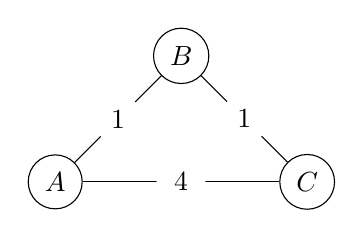
\begin{tikzpicture}[scale=0.8]
			\node[circle, draw] (A) at (0, 0) {$A$};
			\node[circle, draw] (B) at (2, 2) {$B$};
			\node[circle, draw] (C) at (4, 0) {$C$};
			\path (A) edge node[fill=white,circle] {$1$} (B);
			\path (B) edge node[fill=white,circle] {$1$} (C);
			\path (A) edge node[fill=white,circle] {$4$} (C);
		\end{tikzpicture}
\end{center}
\item
درست. می‌دانیم الگوریتم $A^*$ همه گره‌ها مانند $x$ را بسط می‌دهد که هزینه ارزیابی آنها حداکثر هزینه ارزیابی گره هدف باشد؛ یعنی اگر $n$ گره هدف باشد، 
$f(x) \leq f(n) = g(n)$. 
اما چون
$g(x) \leq g(x) + h(x) = f(x)$
پس 
$g(x) \leq g(n)$. 
بنابر شرایط گفته شده 
$g(n)$
بهینه است و در نتیجه گره $x$ توسط الگوریتم 
\lr{Uniform Cost Search}
نیز بسط داده می‌شود چرا که این الگوریتم همه گره‌ها با هزینه کمتر از 
$g(n)$
را بسط می‌دهد.
		\item 
		نادرست. مشکل اصلی 
		$A^*$
		پیچیدگی زمانی آن نیست بلکه پیچیدگی فصای مصرفی آن زیاد است. (همان طور که الگوریتم 
		$IDS$
		برای کاهش فضای مصرفی الگوریتم $BFS$ و 
		\lr{completeness}
		الگوریتم $DFS$ ارائه شد.)
			
	\end{enumerate}
		\section*{
		سوال سوم
	}
با توجه به شماره دانشجویی مسئله چهارم را حل می‌کنم. درستی گزاره را ثابت می‌کنیم. فرض کنیم گره $v$ مجاور گره $u$ باشد و هزینه انتقال از $u$ به $v$ برابر $c$ باشد. چون $x$ و $y$ تابع‌هایی 
\lr{consistent}
هستند، خواهیم داشت:
\begin{align*}
	&x(u) \leq c + x(v) \\
	&y(u) \leq c + y(v)
\end{align*}
نامساوی اول را در $\alpha$ و نامساوی دوم را در 
$1 - \alpha$
ضرب می‌کنیم: (دقت کنید به دلیل برقراری شرط $0 < \alpha < 1$ می‌توانیم بدون تغییر جهت نامساوی این کار را انجام دهیم.)
\begin{align*}
	\alpha x(u) &\leq \alpha c + \alpha x(v) \\
	(1- \alpha)y(u) &\leq (1- \alpha) c + (1- \alpha) y(v)
\end{align*}
با جمع روابط بالا داریم:
$$\alpha x(u) + (1- \alpha)y(u) \leq c + \alpha x(v) + (1- \alpha) y(v)$$
که حکم نتیجه می‌شود.
	\section*{
		سوال چهارم
	}
	مسئله اول را حل می‌‌کنیم.
	\begin{enumerate}
		\item 
		هر حالت قرارگیری $n$ پکمن در $m$ خانه نقشه یک حالت یا 
		\lr{state}
		خواهد بود. همچنین بین هر دو حالت 
		\lr{reachable}
		یک 
		\lr{transition}
		وجود دارد.
		\item 
		با توجه به بخش قبل و فرض مسئله که امکان قرارگیری چندین پکمن در یک خانه از نقشه وجود دارد، می‌توان گفت اندازه فضای حالت برابر 
		$m^n$
		خواهد بود چرا که هر پکمن می‌تواند در یکی از $m$ خانه نقشه قرار گیرد.
		\item 
		در صورتی که موقعیت همه پکمن‌ها به گونه‌ای باشد که بتوانند در هر چهار جهت بالا، پایین، چپ و راست حرکت کنند و همچنین بتوانند در جای خود باقی بمانند، تعداد یال‌های خروجی هر حالت برابر 
		$b \leq 5^n - 1$
		خواهد بود. (دقت کنید حداقل یک پکمن باید حرکت کند. در غیر این صورت درجا می‌زنیم. یک واحد به این دلیل کسر شده است.) به وضوح در صورت قرارگیری پکمن‌ها در حاشیه و مرز نقشه تعداد یال‌های خروجی آن حالت یا 
		\lr{branching factor}
		از $b$ کمتر خواهد بود. همچنین کران پایین 
		$2^n - 1 \leq b$
		را نیز داریم چرا که هر پکمن یا یک خانه مجاور دارد (اگر نقشه همبند باشد.) یا می‌تواند در جای خود باقی بماند. 
		\item 
		در این مسئله تابع هزینه گام‌های مسئله 
	\LTRfootnote{Step cost function}
		عددی صحیح بین 1 و $n$ است چرا که حداقل یک پکمن یک گام حرکت کرده و همچنین حداکثر همه پکمن‌ها هر کدام یک گام حرکت می‌کنند. می‌دانیم در الگوریتم
		\lr{Uniform Cost Search}
حداکثر همه گره‌هایی بسط داده می‌شوند که مسیر بهینه آنها هزینه‌ای کمتر از پاسخ بهینه مسئله ($ C^* $) را دارد. چون تابع هزینه حداقل $\epsilon = 1$ است پس حداکثر همه گره‌ها تا عمق 
$d = \lfloor\frac{C^*}{\epsilon}\rfloor + 1 = C^* + 1$
\footnote{
دلیل وجود یک در این عبارت این است که الگوریتم 
\lr{UCS}
زمانی خاتمه می‌یابد که گره هدف را از صف اولویت خارج کند و قبل از بسط آن، هدف بودن آن را بررسی می‌کند و نه زمانی که آن را ایجاد می‌کند.
}
بسط داده می‌شوند؛ یعنی حداکثر
$b + b^2 + \cdots + b^d = \frac{b(b^{d} - 1)}{b - 1}$
گره. با توجه به بخش قبل $b$ کران پایین بزرگی دارد و می‌توانیم فرض کنیم عبارت بالا از 
$b^d$
کمتر است. از طرفی در این مسئله هر گره هدف حداکثر در عمق 
$m - 1$
خواهد بود زیرا محدودیتی برای تعداد پکمن‌هایی که می‌توانند همزمان در یک خانه از نقشه قرار داشته باشند نداریم و هر پکمن با پیمایش این تعداد گام همه‌ی خانه‌های نقشه را یک بار مشاهده می‌کند. همچنین تابع هزینه هر گام حداکثر $n$ خواهد بود. پس 
$C^* \leq n (m-1)$.
به کمک بخش قبل داریم 
$b^d \leq (5^n - 1)^{n (m-1) + 1}$.
		
	\item
	این تابع هر دو شرایط را دارد. ابتدا ثابت می‌‌کنیم تابع 
	\lr{admissible}
	است؛ یعنی تابع هیوریستیک، از هزینه واقعی بیشتر نیست. اگر مستطیل
	$R = [X_1, X_2] \times [Y_1, Y_2]$
	مستطیلی با کمترین مساحت باشد که همه پکمن‌ها درون یا روی آن قرار بگیرند، (چپ‌ترین پکمن روی خط $ x = X_1 $، راست‌ترین پکمن روی خط $ x = X_2 $، پایین‌ترین پکمن روی خط $ y = Y_1 $ و بالاترین پکمن روی خط $ y = Y_2 $ قرار می‌گیرند.) تابع هیوریستیک برابر 
	$h = \frac{1}{2}\max(X_2 - X_1, Y_2 - Y_1)$
	خواهد بود. بدون کاسته شدن از کلیت مسئله اگر 
	$h = \frac{1}{2}(X_2 - X_1)$
	و همچنین جواب بهینه برای این مسئله، ملاقات پکمن‌ها در نقطه 
	$(\alpha, \beta)$
	باشد، در این صورت اگر $\alpha \leq \frac{X_1 + X_2}{2}$، فاصله منهتن 
	\LTRfootnote{Manhattan distance}
	پکمن روی خط 
	$x = X_2$
	حداقل $h$ خواهد بود و اگر $\alpha \geq \frac{X_1 + X_2}{2}$، فاصله منهتن پکمن روی خط 
	$x = X_1$
	حداقل $h$ خواهد بود. به طوری مشابه برای 
	$h = \frac{1}{2}(Y_2 - Y_1)$
	نیز ثابت می‌شود ک $h$ کران پایینی برای هزینه واقعی حل مسئله خواهد بود.
	
	اکنون ثابت می‌کنیم تابع هیوریستیک 
	\lr{consistent}
	است. اگر $v$ گره‌ی مجاور گره‌ی $u$ باشد و هزینه انتقال از $u$ به $v$ برابر $c$ باشد، نشان می‌دهیم 
	$h(u) \leq h(v) + c$.
مستطیل‌های $ R_u $ و $ R_v $ را مانند اثبات قبل به ترتیب برای وضعیت‌های $u$ و $v$ تعریف می‌کنیم. (مستطیل‌هایی با کمترین مساحت و اضلاع موازی محور‌های مختصات که پکمن‌ها درون یا روی آنها قرار دارند.) همچنین اندازه طول مستطیل $R$ را با $L(R)$ و اندازه عرض آن را با $W(R)$ نشان می‌دهیم. بدون کاسته شدن از کلیت مسئله فرض کنیم 
	$L(R_u) \geq W(R_u)$
و در نتیجه 
$h(u) = \frac{L(R_u)}{2}$.
چون طول گام پکمن‌ها یک واحد است،
$|L(R_u) - L(R_v)| \leq 2$
و
$|W(R_u) - W(R_v)| \leq 2$
چرا که پکمن‌های روی طول یا عرض $R_u$ می‌توانند به سمت یکدیگر یا خلاف همدیگر حرکت کنند. در نتیجه 
$|h(u) - h(v)| \leq 1$.
 اگر $h(u) - h(v) = 1$، چون $ c \geq 1 $ آنگاه 
 $h(u) \leq h(v) + c$. 
 در غیر این صورت (مثلا $h(v) \geq h(u)$) رابطه
  $h(u) < h(v) + c$
   برقرار خواهد بود. پس در هر صورت داریم 
   $h(u) \leq h(v) + c$.

	\end{enumerate}
					\section*{
			گزارش پروژه
		}
	بخش اصلی پروژه در ماژول 
	\code{puzzle.py}
	قرار دارد و ماژول‌
	\code{priority_queue.py}
	پیاده سازی صف اولویت است که مستقیما از کدهای کتاب ساختمان داده گودریخ و تاماسیا
	\cite[فصل ۹]{goodrich2013data}
	که در 
	\href{https://higheredbcs.wiley.com/legacy/college/goodrich/1118290275/dsap/ch09.zip}{اینجا}
	قرار داده شده‌اند استفاده شده است. (دلیل عدم استفاده از کتابخانه \code{heapq} در ادامه گفته می‌شود.) برای پیاده سازی از سه کلاس \code{State}، \code{Node} و \code{Puzzle} استفاده شده است. نمونه‌های کلاس 
	\code{State}
	همگی
	\lr{hashable}
	هستند زیرا لازم است بتوان آنها را به عنوان کلید در ساختمان داده‌های
	\code{dict}
	و
	\code{set}
	به کار برد. بدین منظور توابع
	\code{__eq__()}
	و
	\code{__hash__()}
	آنها 
	\lr{override}
	شده‌اند. تابع 
	\code{__hash__()}
	ماتریس حالت را به 
	\code{tuple}
	تبدیل می‌کند و سپش هش آن را برمی‌گرداند. (شایان ذکر است که برای کاسته شدن از سربار تبدیل ماتریس حالت به چندتایی، آن را یک بار و هنگام مقدار دهی اولیه ایجاد کرده و ذخیره می‌کنیم.) تابع 
	\code{find_position()}
	که 
	\lr{public}
	است، موقعیت هر سلول (در این پیاده سازی سلول‌ها می‌تواند عدد، رشته یا هر شی دیگری باشند.) که به آن ورودی داده شود را محاسبه می‌کند. سلول خالی را با 
	\code{None}
	نشان می‌دهیم. نمونه‌های کلاس 
	\code{State}
	را می‌توان به کمک ماتریس حالت ایجاد کرد. تابع
	\code{actions()}
	که
	\lr{protected}
	است، حرکات مجاز سلول خالی را به صورت لیستی از \code{Action}ها برمی‌گرداند. سپس تابع 
	\code{adjacent_states()}
که \lr{public} است، حالت‌هایی که به کمک این حرکات مجاز قابل دسترسی هستند را به صورت لیستی از \code{State}ها برمی‌گرداند.
\begin{latin}
\begin{lstlisting}
class State:
	def __init__(self, state_matrix: List[List]):
		union = []
		for row in state_matrix:
			union.extend(row)
		self.__state_tuple: tuple = tuple(union)
		self.__state_matrix = state_matrix
	
	def to_tuple(self) -> tuple:
		return self.__state_tuple
	
	def __hash__(self):
		return hash(self.__state_tuple)
	
	def __eq__(self, other):
		return other.to_tuple() == self.__state_tuple
	
	def find_position(self, x) -> (int, int):
		for i in range(len(self.__state_matrix)):
			if x in self.__state_matrix[i]:
				return i, self.__state_matrix[i].index(x)
	
	def __actions(self) -> List[Action]:
		i, j = self.find_position(None)
		n = len(self.__state_matrix) - 1
		result = []
		if j != 0:
			result.append(Action.Left)
		if j != n:
			result.append(Action.Right)
		if i != 0:
			result.append(Action.Up)
		if i != n:
			result.append(Action.Down)
		return result
	
	def adjacent_states(self):
		i, j = self.find_position(None)
		result = []
		for action in self.__actions():
			x = deepcopy(self.__state_matrix)
			if action == Action.Up:
				x[i - 1][j], x[i][j] = x[i][j], x[i - 1][j]
			elif action == Action.Down:
				x[i + 1][j], x[i][j] = x[i][j], x[i + 1][j]
			elif action == Action.Right:
				x[i][j + 1], x[i][j] = x[i][j], x[i][j + 1]
			elif action == Action.Left:
				x[i][j - 1], x[i][j] = x[i][j], x[i][j - 1]
			result.append((State(x), action))
		return result
\end{lstlisting}
\end{latin}

 کلاس 
\code{Node}
نماینگر یک گره است که برای پیمایش الگوریتم
$A^*$
 به کار می‌رود و هزینه هیوریستیک، کل هزینه تخمین زده شده و همچنین هزینه مسیر از گره شروع تا گره فعلی را ذخیره سازی می‌کند. آدرس گره والد، حالت مسئله در گره فعلی و نوع حرکت انجام شده برای انتقال از حالت متناظر گره والد به حالت نظیر گره فعلی نیز در این کلاس ذخیره می‌شود.
\begin{latin}
\begin{lstlisting}
class Node:
	def __init__(self, state: State, g_cost: int, h_cost: int, 
				 parent, action: Action | None):
		self.parent = parent
		self.state: State = state
		self.f_cost: int = g_cost + h_cost
		self.g_cost: int = g_cost
		self.h_cost: int = h_cost
		self.action: Action = action
\end{lstlisting}
\end{latin}
 
  نمونه‌های کلاس 
 \code{Puzzle}
 با دو ماتریس متناظر حالت شروع و حالت هدف مقدار دهی اولیه می‌شوند. این ماتریس‌ها بلافاصله به صورت 
 \code{State}
 ذخیره می‌شوند. همچنین یک 
 \code{dict}
 از سلول‌ها و موقعیت آنها در ماتریس حالت هدف ایجاد می‌شود. کاربرد این 
 \lr{dictionary}
 در تابع 
 \code{heuristic(state: State)}
 است که 
 \lr{private}
 است. در واقع تابع هیوریستیک با ورودی گرفتن یک حالت، به کمک تابع
 \code{manhattan_distance(t1: (int, int), t2: (int, int))}
 مجموع فاصله منهتن بین هر سلول در حالت هدف و حالت داده شده \code{state} را محاسبه می‌کند.
\begin{latin}
\begin{lstlisting}
class Puzzle:
	def __init__(self, initial_state_matrix: List[List], 
				 goal_state_matrix: List[List]):
		self.__initial_state = State(initial_state_matrix)
		self.__goal_state = State(goal_state_matrix)
		self.__goal_state_cells_positions = {
			cell: self.__goal_state.find_position(cell)
			for cell in self.__goal_state.to_tuple() if cell is not None
		}

	def __heuristic(self, state: State) -> int:
		s = 0
		for cell, goal_position in self.__goal_state_cells_positions.items():
			s += self.__manhattan_distance(
				state.find_position(cell), 
				goal_position
			)
		return s

	@staticmethod
	def __manhattan_distance(t1: (int, int), t2: (int, int)) -> int:
		return abs(t1[0] - t2[0]) + abs(t1[1] - t2[1])
\end{lstlisting}
\end{latin}
 
  الگوریتم 
 $A^*$
 در تابع
 \code{solve()}
 کلاس 
 \code{Puzzle}
 پیاده سازی شده است که کد آن را در زیر می‌بینید. این الگوریتم مانند الگوریتم
 \lr{Uniform Cost Search}
 یا 
 \lr{Dijkstra}
 پیاده سازی شده است.
\begin{latin}
\begin{lstlisting}
def solve(self) -> List[Node] | None:
	frontier = AdaptableHeapPriorityQueue()
	explored = set()
	frontier_nodes_by_states = {}
	frontier_locators_by_nodes = {}
	initial_node = Node(
		self.__initial_state,
		0,  # initial g_cost is 0
		self.__heuristic(self.__initial_state),
		None,
		None
	)
	add_to_frontier(initial_node.f_cost, initial_node)
	while not frontier.is_empty():
		key, node = frontier.remove_min()
		remove_from_frontier_finders(node)
		if self.__is_goal_state(node.state):
			return self.__solution(node)
		explored.add(node.state)
		for child in self.__children(node):
			if child.state not in explored and \
					child.state not in frontier_nodes_by_states:
				add_to_frontier(child.f_cost, child)
			elif child.state in frontier_nodes_by_states:
				suspect = frontier_nodes_by_states[child.state]
				if suspect.f_cost > child.f_cost:
					suspect_locator = frontier_locators_by_nodes[suspect]
					remove_from_frontier_finders(suspect)
                    update_frontier(suspect_locator, child.f_cost, child)
	return None
\end{lstlisting}
\end{latin}
 همان طور که مشخص است دو 
 \lr{dictionary}
 به نام‌های 
 \code{frontier_nodes_by_states}
 و
 \code{frontier_locators_by_nodes}
 تعریف شده است که اولی اجازه می‌دهد گره‌ای درون صف اولیت که نظیر یک حالت از مسئله است را پیدا کنیم. (خط ۲۲ را ببینید.) دومی اجازه می‌دهد به 
 \lr{locator}
 یک گره درون صف اولویت دسترسی پیدا کنیم. (خط ۲۷ را ببینید.) در واقع به کمک 
  \lr{locator}
  در پیاده سازی 
  \code{AdaptableHeapPriorityQueue()}
 می‌توان کلید یک گره در صف اولویت را بروزرسانی کرد یا یک گره دلخواه را از صف اولویت خارج کرد. این همان دلیل استفاده از این صف اولویت به جای کتابخانه 
 \code{heapq}
 است. در واقع در صورت برقراری شرط خط ۲۶، مسیری با هزینه کمتری برای گره 
 \code{suspect}
 پیدا شده است. در نتیجه به کمک 
 \lr{locator}
 آن، این گره از صف اولویت خارج شده و گره 
 \code{child}
 که همان وضعیت مسئله را دارد ولی هزینه کمتری دارد جایگزین آن می‌شود. (این عملیات به صورت بروزرسانی همزمان کلید و گره در خط ۲۹ پیاده سازی شده است.) همچنین چهار 
 \lr{inner function}
 به نام‌های
 \code{add_to_frontier}،
 \code{add_to_frontier_finders}،
 \code{remove_from_frontier_finders}
 و
 \code{update_frontier}
 برای هماهنگی
 \code{frontier}،
 \code{frontier_nodes_by_states}
 و
 \code{frontier_locators_by_nodes}
 نوشته شده‌اند.
\begin{latin}
\begin{lstlisting}
def add_to_frontier_finders(locator, node: Node):
	frontier_nodes_by_states[node.state] = node
	frontier_locators_by_nodes[node] = locator
	
def add_to_frontier(f_cost: int, node: Node):
	locator = frontier.add(f_cost, node)
	add_to_frontier_finders(locator, node)
	
def remove_from_frontier_finders(node: Node):
	del frontier_nodes_by_states[node.state]
	del frontier_locators_by_nodes[node]
	
def update_frontier(locator, f_cost: int, node: Node):
	frontier.update(locator, f_cost, node)
	add_to_frontier_finders(locator, node)	
\end{lstlisting}
\end{latin}
هنگامی که الگوریتم گره هدف را از صف اولویت خارج کند یعنی همه گره‌ها با هزینه کوچکتر از 
$f(goal)$
گسترش داده شده‌اند و مسیر بهینه گره هدف پیدا شده است.

 در این صورت به کمک تابع 
\code{solution(goal_node: Node)}
 و تابع بازگشتی
\code{recursively_find_solution(node: Node)}
مسیر حرکت از گره شروع به گره هدف را به کمک آدرس گره والد پیدا می‌کنیم. 
\begin{latin}
\begin{lstlisting}
def __recursively_find_solution(self, node: Node) -> List[Node]:
	if node.parent is None:
		return [node]
	path = self.__recursively_find_solution(node.parent)
	path.append(node)
	return path

def __solution(self, goal_node: Node) -> List[Node]:
	return self.__recursively_find_solution(goal_node)
\end{lstlisting}
\end{latin}

همچنین تابع
\code{children(parent_node: Node)}
گره‌های مجاور گره والد را به کمک تابع
\code{adjacent_states()}
ایجاد می‌کند. 

تابع
\code{child_node(parent_node: Node, child_state: State, action: Action)}
با ورودی گرفتن گره والد و حالت فرزند، یک گره با هزینه‌های 
$g(child) = g(parent) + 1$
و
$f(child) = g(child) + h(child)$
برمی‌گرداند.
\begin{latin}
\begin{lstlisting}
def __children(self, parent_node: Node) -> List[Node]:
	return [
		self.__child_node(parent_node, child_state, action)
		for child_state, action in parent_node.state.adjacent_states()
	]

def __child_node(self, parent_node: Node, child_state: State, 
				 action: Action) -> Node:
	return Node(
		child_state,
		parent_node.g_cost + 1,  # step cost is 1
		self.__heuristic(child_state),
		parent_node,
		action
	)
\end{lstlisting}
\end{latin}
چون اینجا الگوریتم 
$A^*$
را روی گراف حالت‌ها پیاده سازی کردیم  و بنابر قضیه کتاب
\cite[صفحه ۹۵ فصل سوم]{russell2010artificial}
برای داشتن جواب بهینه باید تابع هیوریستیک
\lr{consistent}
باشد. اثبات این موضوع ساده است چرا که اگر $v$ گره مجاور $u$ باشد، هزینه انتقال از $u$ به $v$ برابر یک خواهد بود و همچنین 
$h(v)$
حداکثر یک واحد کمتر از 
$h(u)$
خواهد بود زیرا فاصله منهتن عدد مجاور مربع خالی می‌تواند حداکثر یک واحد کاهش یابد یا به عبارتی نزدیک هدف شود و این حرکت در فاصله منهتن مابقی اعداد تاثیری ندارد.
	\setLTRbibitems
	\bibliography{refs.bib}
\end{document}